\section{Risultati}\label{sec:risultati}
  I risultati ottenuti sono riassunti nelle tabelle \ref{tab : risultati} e \ref{tab : risultati-beta}. I valori numerici dei dati raccolti sono riportati in appendice \ref{sec:valori-misure}. Il grafico in figura \ref{fig : dati raccolti} rappresenta le osservazioni effettuate con sovraimpressi i \emph{fit}.
  \begin{table}[H]
    \centering
    \begin{tabular}[t]{c | c  c  c }
      \hline
      & $-100 \: \mu A$ & $-150 \: \mu A$ & $-200\: \mu A$ \\
      \hline
      Conduttività & $(17.81 \pm 0.06) \: \Omega^{-1}$ & $(24.34 \pm 0.08) \: \Omega^{-1}$ & $(30.62 \pm 0.11) \: \Omega^{-1}$ \\
      Tensione di Early & $(0.0561 \pm 0.0019) \: V$ & $(0.0534 \pm 0.0018) \: V$ & $(0.0627 \pm 0.0019) \: V$ \\
      \hline
    \end{tabular}
    \caption{\emph{Valori di caratteristica misurati e rispettivi valori di corrente di base.}}
    \label{tab : risultati}
  \end{table}
  \begin{table}[H]
    \centering
    \begin{tabular}[t]{c | c  c  c }
      \hline
      $\left|I_{B2} - I_{B1}\right|$ & $(150 - 100) \: \mu A$ & $(200 - 150) \: \mu A$ & $(200 - 100)\: \mu A$ \\
      \hline
      $\beta$ ($-3 \: V$) & $149 \pm 12$ & $159 \pm 14$ & $308 \pm 12$ \\
      \hline
    \end{tabular}
    \caption{\emph{Valori di $\beta$ calcolati per un valore fissato di $V_{CE} = -3V$. Le incertezze su $\beta$ sono ottenute sommando
    linearmente le incertezze per $\Delta I_B$ e $\Delta I_C$.}}
    \label{tab : risultati-beta}
  \end{table}

  \begin{figure}[h]
    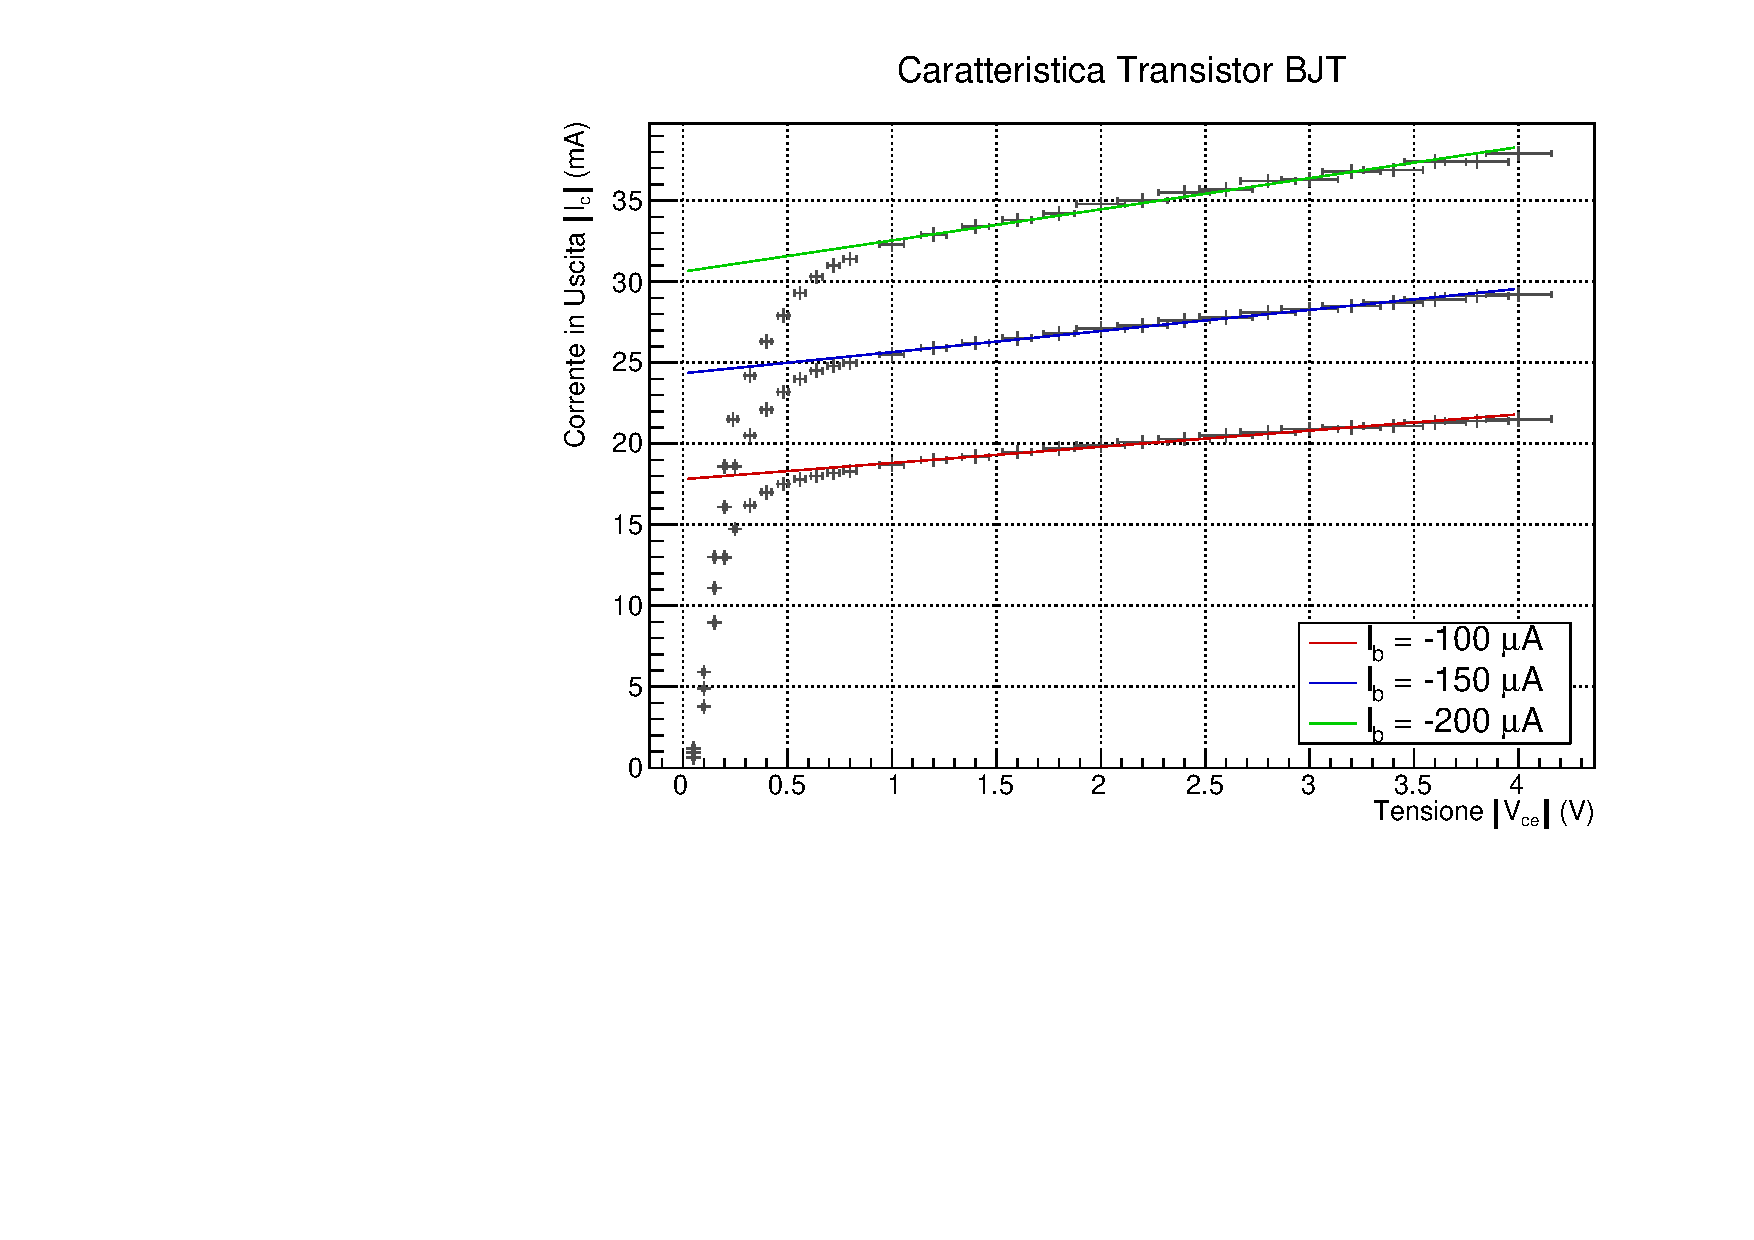
\includegraphics[width=\textwidth]{../assets/GraficoTot.pdf}
    \caption{\emph{Dati raccolti con relativo fit lineare. In tutti e tre i casi il fit è stato svolto per valori di tensione $\left|V_{ce}\right| \geq 1$.}}
    \label{fig : dati raccolti}
  \end{figure}
